\section{Design}
\label{sec:design}

Around 5 pages about functional aspects of the FeedApp application.

Concretely, you shall write about 

\begin{itemize}
	\item the \emph{use cases},
	\item the \emph{domain model}, and
	\item the \emph{architecture} (including applied technologies)
\end{itemize}

Each part shall ideally be accompanied with a graphical representation (diagram).

You may have a look at the \href{https://github.com/selabhvl/dat250public/blob/master/projectdescription/README.md}{Examples on GitHub}.




\subsection{Use cases}

The purpose of a use case diagram is to outline the functionalities the system will implement, identify the various roles involved, and specify where user interfaces are needed. The UML provides a high-level view of system interactions which features are necessary, who will be using them, and how users will access them within the application. 

In the FeedApp application is there two separate roles. First there is the anonymous user. An anonymous user can only view and vote on public polls. They can also register a new account or log in to an existing one. A logged in user can view and vote on every poll. The logged in user can also create a new poll or edit and delete their existing polls.

\begin{figure}[thb]
	\centering
	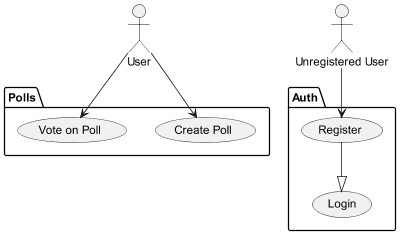
\includegraphics[scale=0.5]{figs/PUML/UseCase.png}
	\label{fig:Use cases}
\end{figure}

Poll availability is decided by the polls author upon creation. 

\subsection{Domain model}

The domain model shows the domain concepts and their relations. A user can have several votes and polls. Each poll have one user who created the poll and two or more poll options. Each of the poll options can have several votes. 

\begin{figure}[thb]
	\centering
	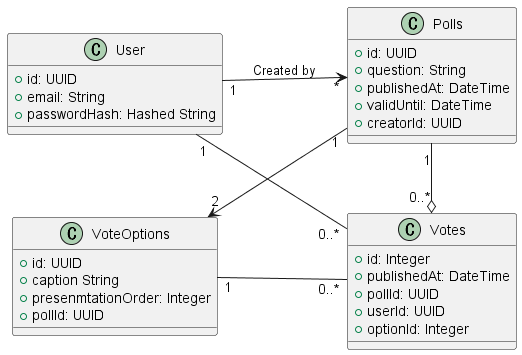
\includegraphics[scale=0.5]{figs/PUML/DomainModel.png}
	\label{fig:Domain model}
\end{figure}

\subsection{System architecture}

For the desing of the FeedApp and the analytic components are several technologies needed. The figure shows the different parts of the app and the technologies used to implement them. For the frontend is Svelte used. 

For the backend is ASP.NET Core used. 


\begin{figure}[thb]
	\centering
	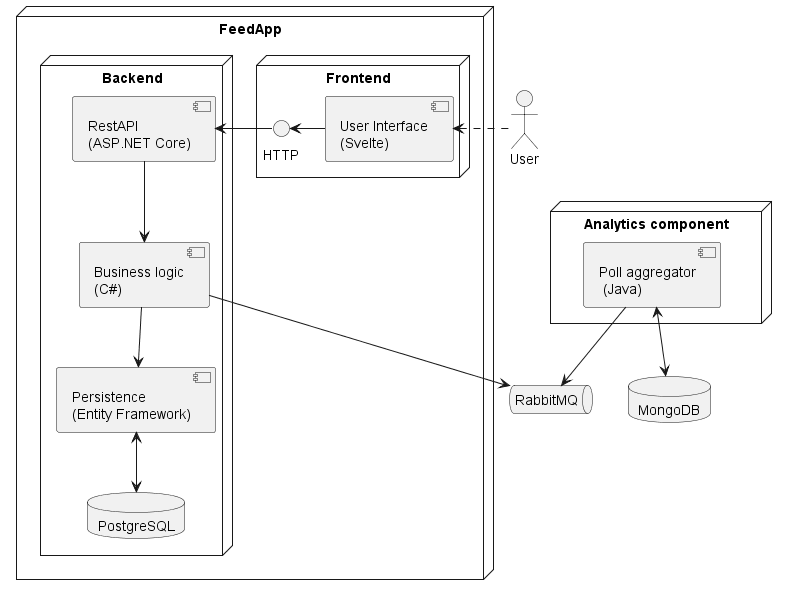
\includegraphics[scale=0.5]{figs/PUML/SystemArchitecture.png}
	\label{fig:System architecture}
\end{figure}

